\section{Evaluation on May 18th}\label{sec:evaluatin_test}
The evaluation of the system and all of its components took place on the 18th of May.
This was conducted as the previous test had not managed to explore the functionality of the game as described in \autoref{sec:initial-test}.
In the time between the two tests, the majority of the discovered bugs were fixed.
Due to the COVID-19 pandemic, the test was conducted using the group members as testers, and only one person from outside the group.

\subsection{The setup}
The test was carried out in two phases, one indoors and one outdoors.
The playing field was shaped like a rectangle for both tests, much like the previous test on the 7th of May as described in \autoref{sec:initial-test}.

\subsection{Method and structure}
The test was largely unstructured, and was to an extent conducted as a big bang test.
Ideally, this test would have been conducted as a usability test, but as the group already had expert knowledge on how to operate the program, it is not possible to test the setup and the usability of the game.
Had a usability test been conducted, it would have been focused on the usage of the system as a player, meaning that a group member would have been in charge of setting up the Pozyx system and running the host computer.
The reason for this is that extensive knowledge about Pozyx is required to set up the game correctly, and that the host program has not been optimized for usability.
Neither of which are things that test subjects would be expected to be able to do.
Instead, they would have been given a short introduction about the game to see if they could understand and play the game, and the group would be present as observers.
Finally, at the end of the usability test, an interview would be conducted to get them to elaborate on their experience, with a special focus on how to make it more user friendly.
Further work into the preparation of a usability test has not been made, as it was deemed impossible to properly conduct the test due to the COVID-19 pandemic.

\subsection{Indoors test}
In the indoor test, the anchors were positioned as seen on \autoref{fig:test2-indoor-setup}.
\begin{figure}[H]
    \centering
    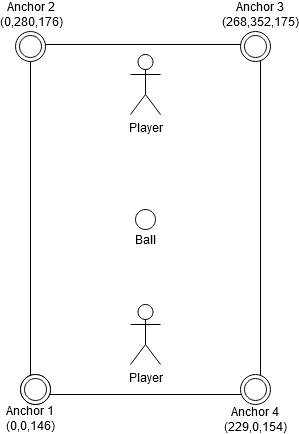
\includegraphics[width=0.5\linewidth]{usability/setupindoors.png}
    \caption{The setup for the indoors playing field. The coordinate at the anchors are in cm.}
    \label{fig:test2-indoor-setup}
\end{figure}
\noindent
During the indoor test it was discovered that two of the Pozyx tags did not correctly send positional updates even though they did not report any problems during the setup phase.
The tags would keep sending error codes that they could not identify themselves or that they could not find enough anchors to calculate their position.
As the two tags continuously kept reporting errors even when being run on a code example made by Pozyx, it was decided that it most likely was a hardware issue and would not be trivial to fix.
\\
The tests were instead successfully carried with one player on each team instead of the intended two players on each team.
The Pozyx positional updates arrived in a timely fashion, and the players were able to play against each other as intended with the remaining two player tags.
An issue in terms of playability was discovered, however.
If the playing field was suitably small, it was difficult for players to pass each other during play.
A picture of the gameplay in progress can be seen on \autoref{fig:usability-test-in-progress}.
\begin{figure}[H]
    \centering
    \includegraphics[width=0.5\linewidth]{usability/usabilitytestindoors.png}
    \caption{Test in progress indoors.}
    \label{fig:usability-test-in-progress}
\end{figure}
\noindent
They could simply just block each other, preventing goals from being scored.
Another point of interest was the inclusion of a physical ball in the design of the game, represented by a single Pozyx tag.
The reason a tag was used to represent the ball is that it seemed unlikely that the tag would be able to send positional data reliably and correctly enough if the tag were to be inserted into a ball since simply blocking the sender on the tag with a finger was enough to block any outgoing signals from it.
Additionally, inserting a tag into a ball and kicking it around could potentially damage the tag if it was not properly fastened securely in position.
Instead, the players were given their player tag and a small power bank to hold in their hands as seen on \autoref{fig:two-tags}, and the ball was attached to a larger power bank such that the players could easily distinguish the two tags even with VR goggles on.

\begin{figure}[H]
    \centering
    \begin{subfigure}{0.45\textwidth}
        \centering
        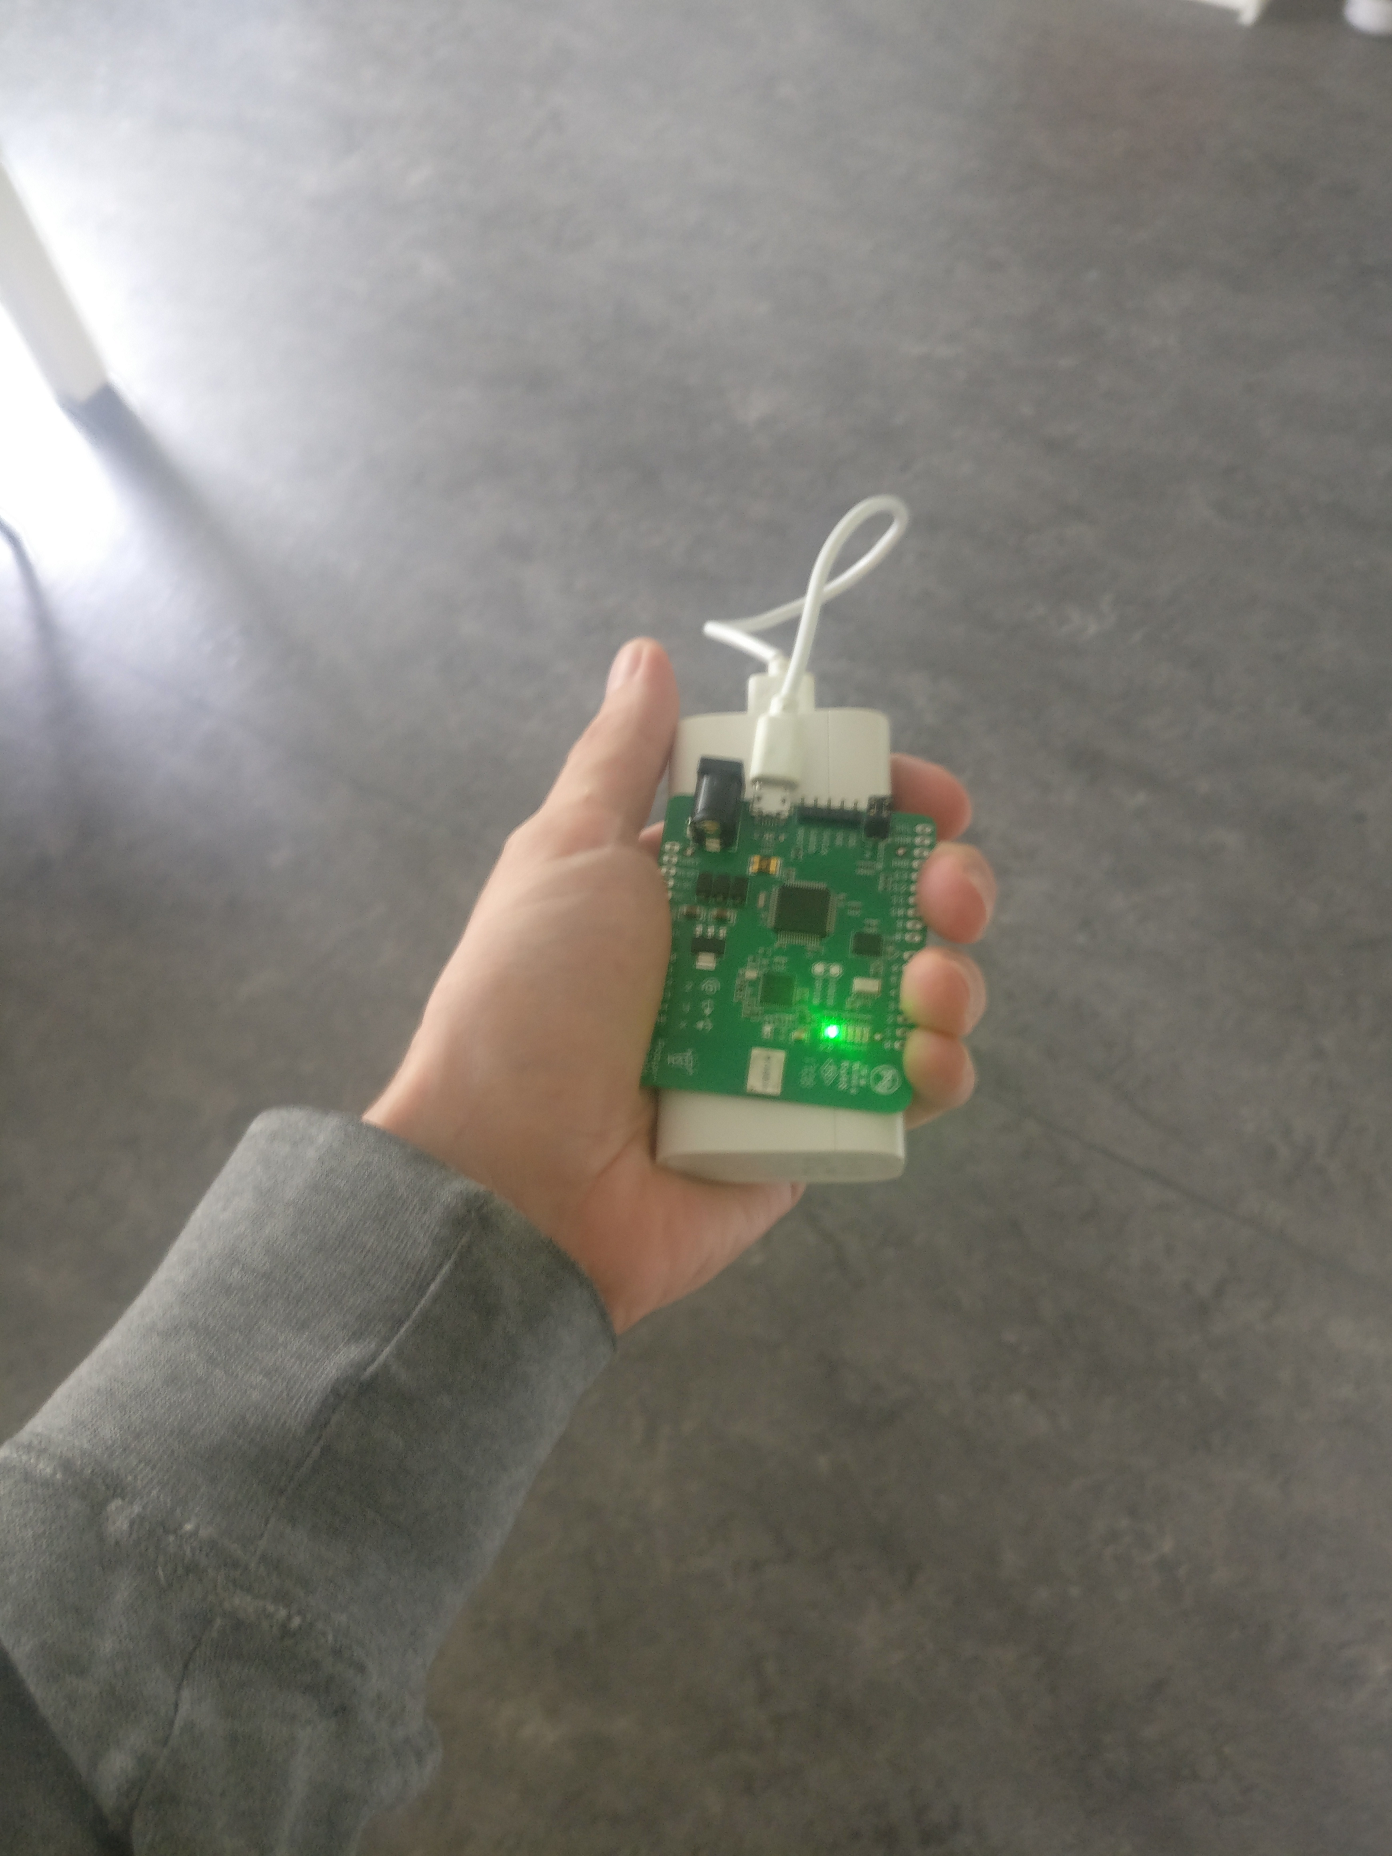
\includegraphics[width=0.8\linewidth]{usability/playertag.png}
        \caption{The player tag and a power bank.}
        \label{fig:sub1}
    \end{subfigure}
    \begin{subfigure}{0.45\textwidth}
        \centering
        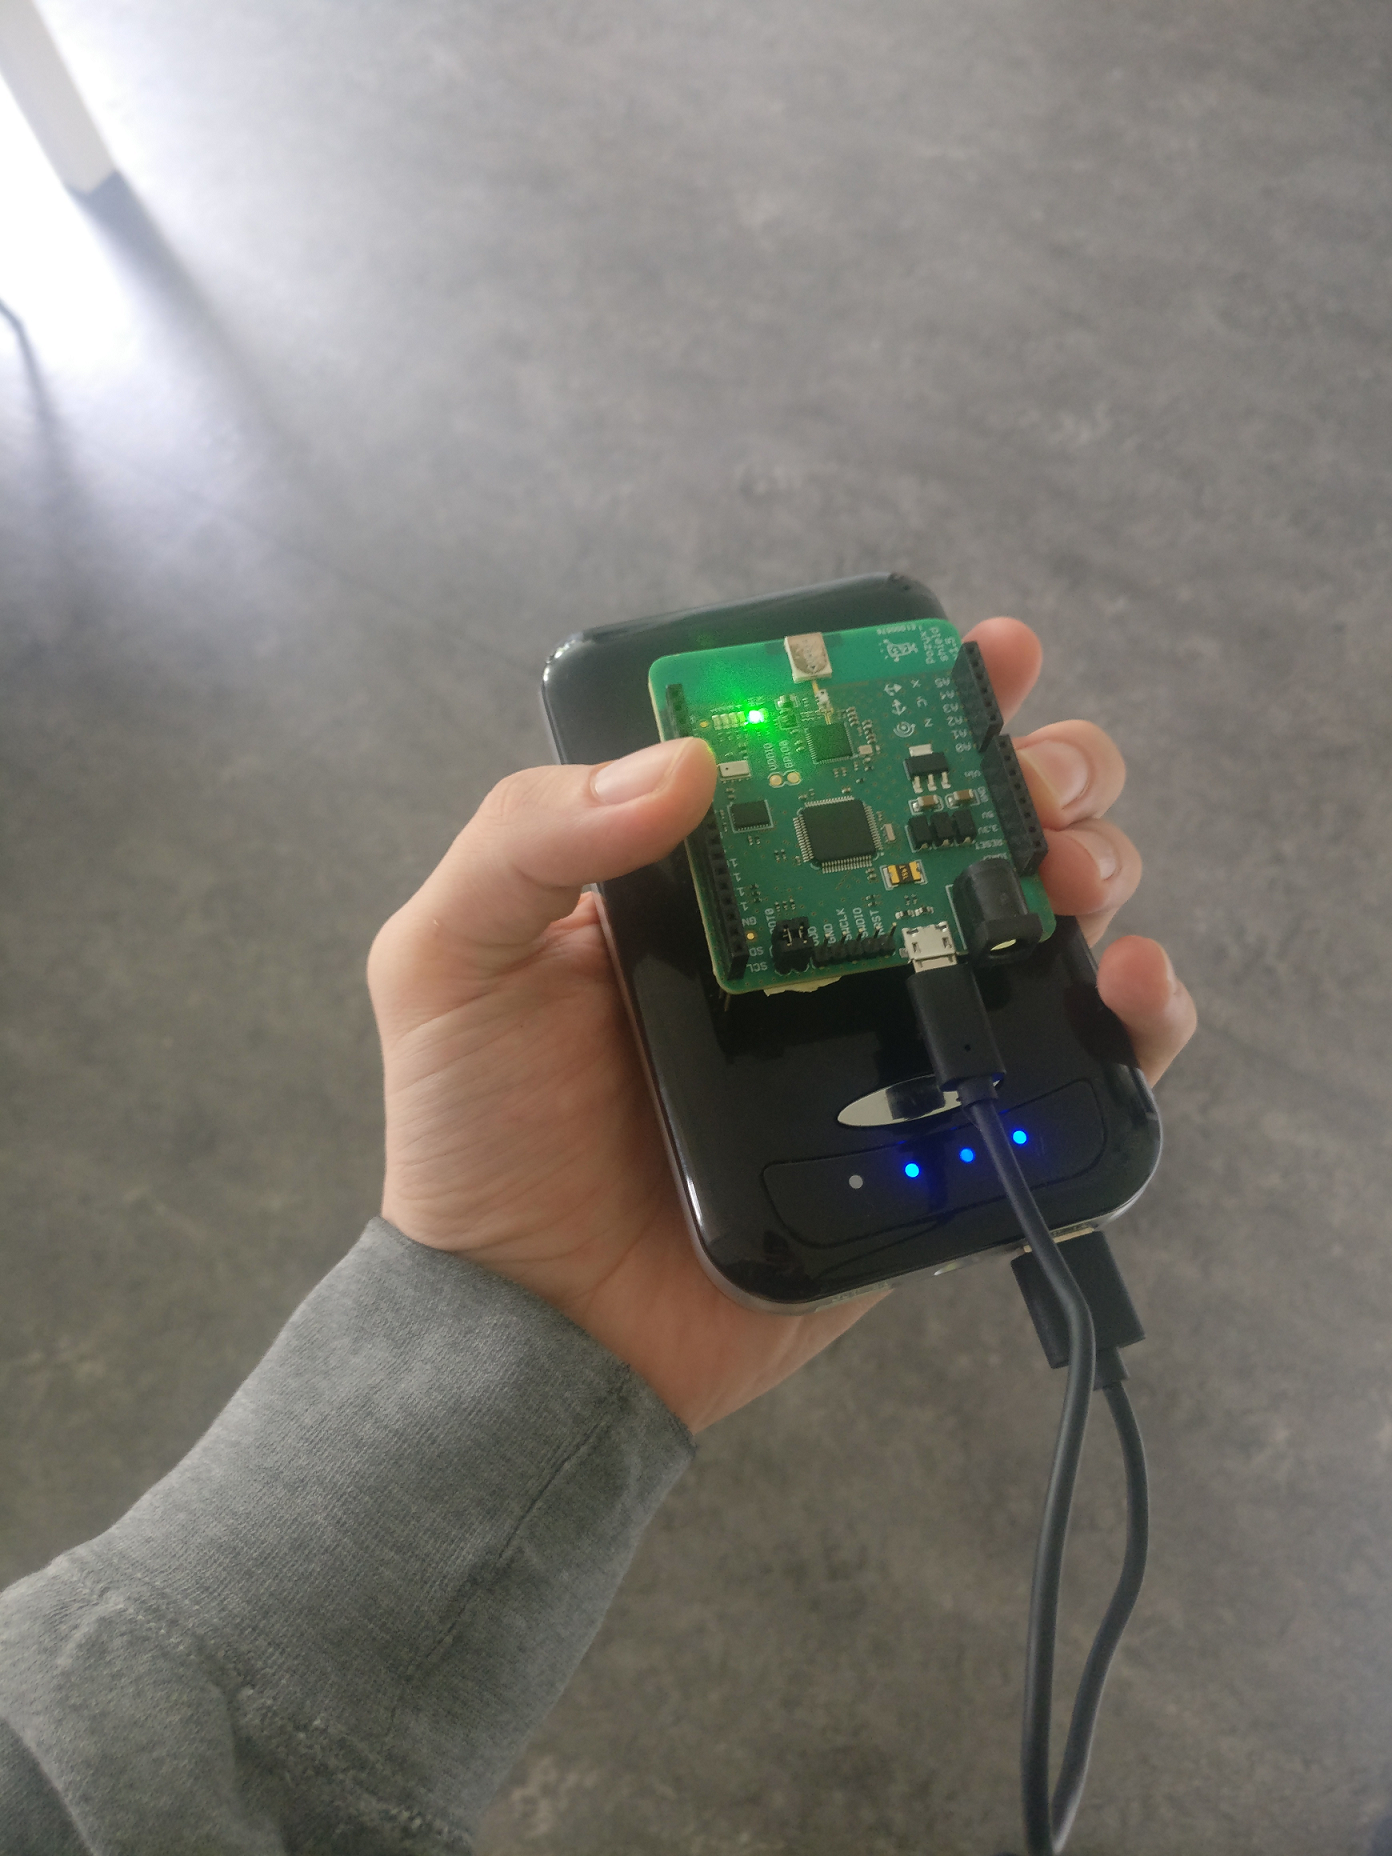
\includegraphics[width=0.8\linewidth]{usability/balltag.png}
        \caption{The ball tag and a power bank.}
        \label{fig:sub2}
    \end{subfigure}
    \caption{The tags used to show positions of players and the ball.}
    \label{fig:two-tags}
\end{figure}
\noindent
For the iteration of the game used for the test, there was no automatic transferal of the ball when players collided, and this is not possible with a physical ball.
As such, an extrinsic rule had to be implemented for further tests.
When colliding, the players would swap possession of the ball, and the player who previously had the ball would count down for a few seconds to allow the new player to gain some distance.
Once this rule had been implemented, the game could be played as intended.

\subsection{Outdoors test}
\begin{figure}[H]
    \centering
    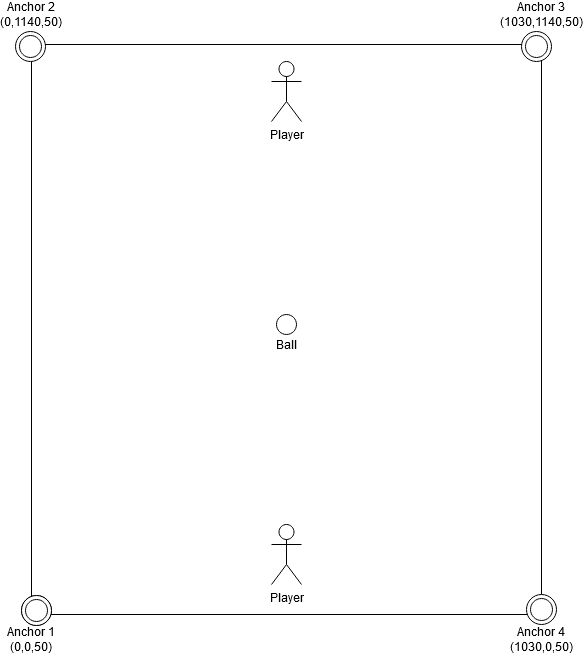
\includegraphics[width=0.5\linewidth]{usability/setupoutdoor.png}
    \caption{The setup for the outdoor playing field. The coordinate at the anchors are in cm.}
    \label{fig:test2-outdoor-setup}
\end{figure}
\noindent
The setup for the outdoor test can be seen on \autoref{fig:test2-outdoor-setup}.
The field was constructed by placing the anchors on top of chairs placed in a rectangular shape, as can be seen on \autoref{fig:test2-anchor-setup}.
\begin{figure}[H]
    \centering
    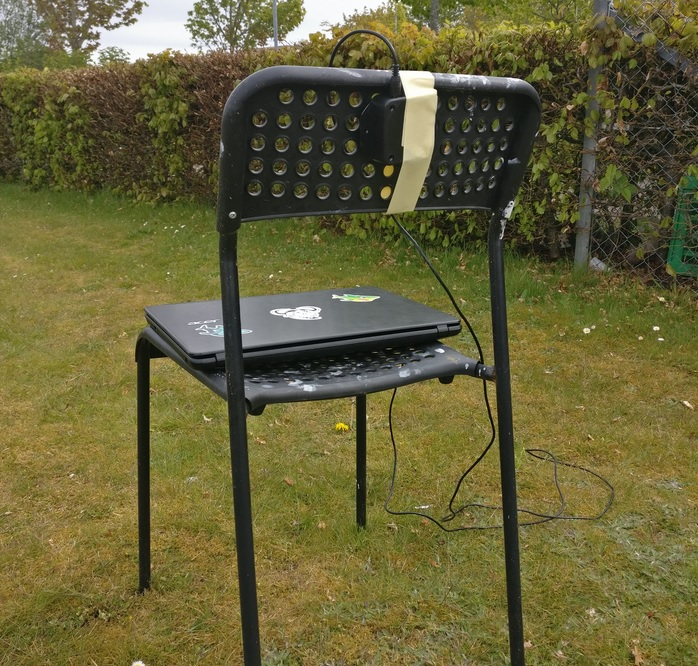
\includegraphics[width=0.4\linewidth]{usability/outdoor-setup.jpg}
    \caption{The setup of an anchor in the outdoor test.}
    \label{fig:test2-anchor-setup}
\end{figure}
\noindent
These anchors were connected to laptops to ensure no components would run out of power during the test.
The game worked fine overall during the outside test, but the testers experienced that the tags sometimes stopped updating for several seconds.
Looking at the debug information available on the host laptop, it was easily seen that it periodically did not send any new positions to the clients, pointing towards a problem with the Pozyx hardware.
The updates of the players' positions would also not update as frequently some times and this could cause the movement of the players to appear quite jerky, and resulted in less positional accuracy compared to the indoor test.
A picture of the gameplay outdoors can be seen on \autoref{fig:outdoor-gameplay}.
\begin{figure}[H]
    \centering
    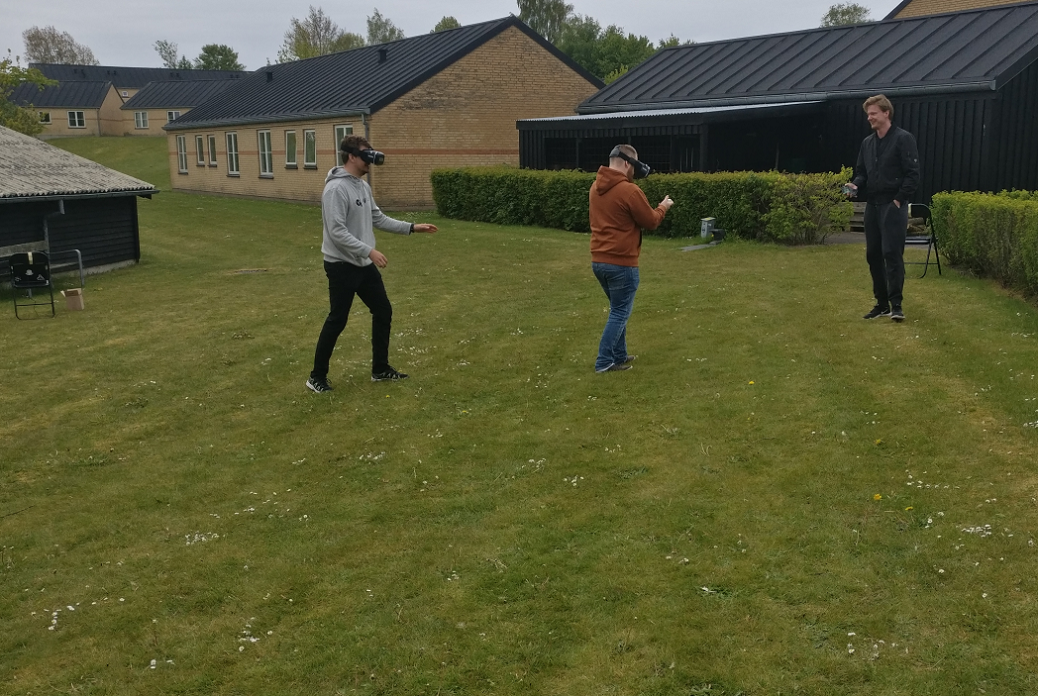
\includegraphics[width=0.6\linewidth]{usability/outdoorusabilitytest.png}
    \caption{Game in progress in the outdoors setup environment.}
    \label{fig:outdoor-gameplay}
\end{figure}

\subsection{Would this meet the users' requirements}
As we were unable to test with more than one external person due to safety concerns related to COVID-19, it is limited how much information was gained from external users.
The external user did, however, have a few comments on the test:

\begin{itemize}
    \item It is impossible to see where you are positioned if you are outside the playing field.
    \item It is very unclear which goal is yours.
    \item It would be good if it was possible to see which direction you are turning.
    \item The update rate was quite slow in the outdoors test and the players are jumping from one position to another
\end{itemize}
Even though the game had a few lacking features, the user was entertained during the test of the game.

\subsubsection{Possible solutions}
There are two primary ways to solve the players not being able to see their position if they are outside the playing field.
The first would be the practical approach, where the field has a physical border to let the players know that they are at the edge.
Alternatively, it would be possible to add some padding around the in-game playing field, so the players can still see themselves until they are a given distance away from the field.
\\
To let the players know which goal is theirs, the player avatars could be colored according to their team color, or the goals could be colored according to their team's avatar.
\\
Letting the players see which direction they are facing could be solved by getting their tag orientation from Pozyx.
To ensure that the tag is always facing the same way as the user, the tag can be mounted on top of the VR goggles as seen on \autoref{fig:tag-on-vr-headset}.

\begin{figure}[H]
    \centering
    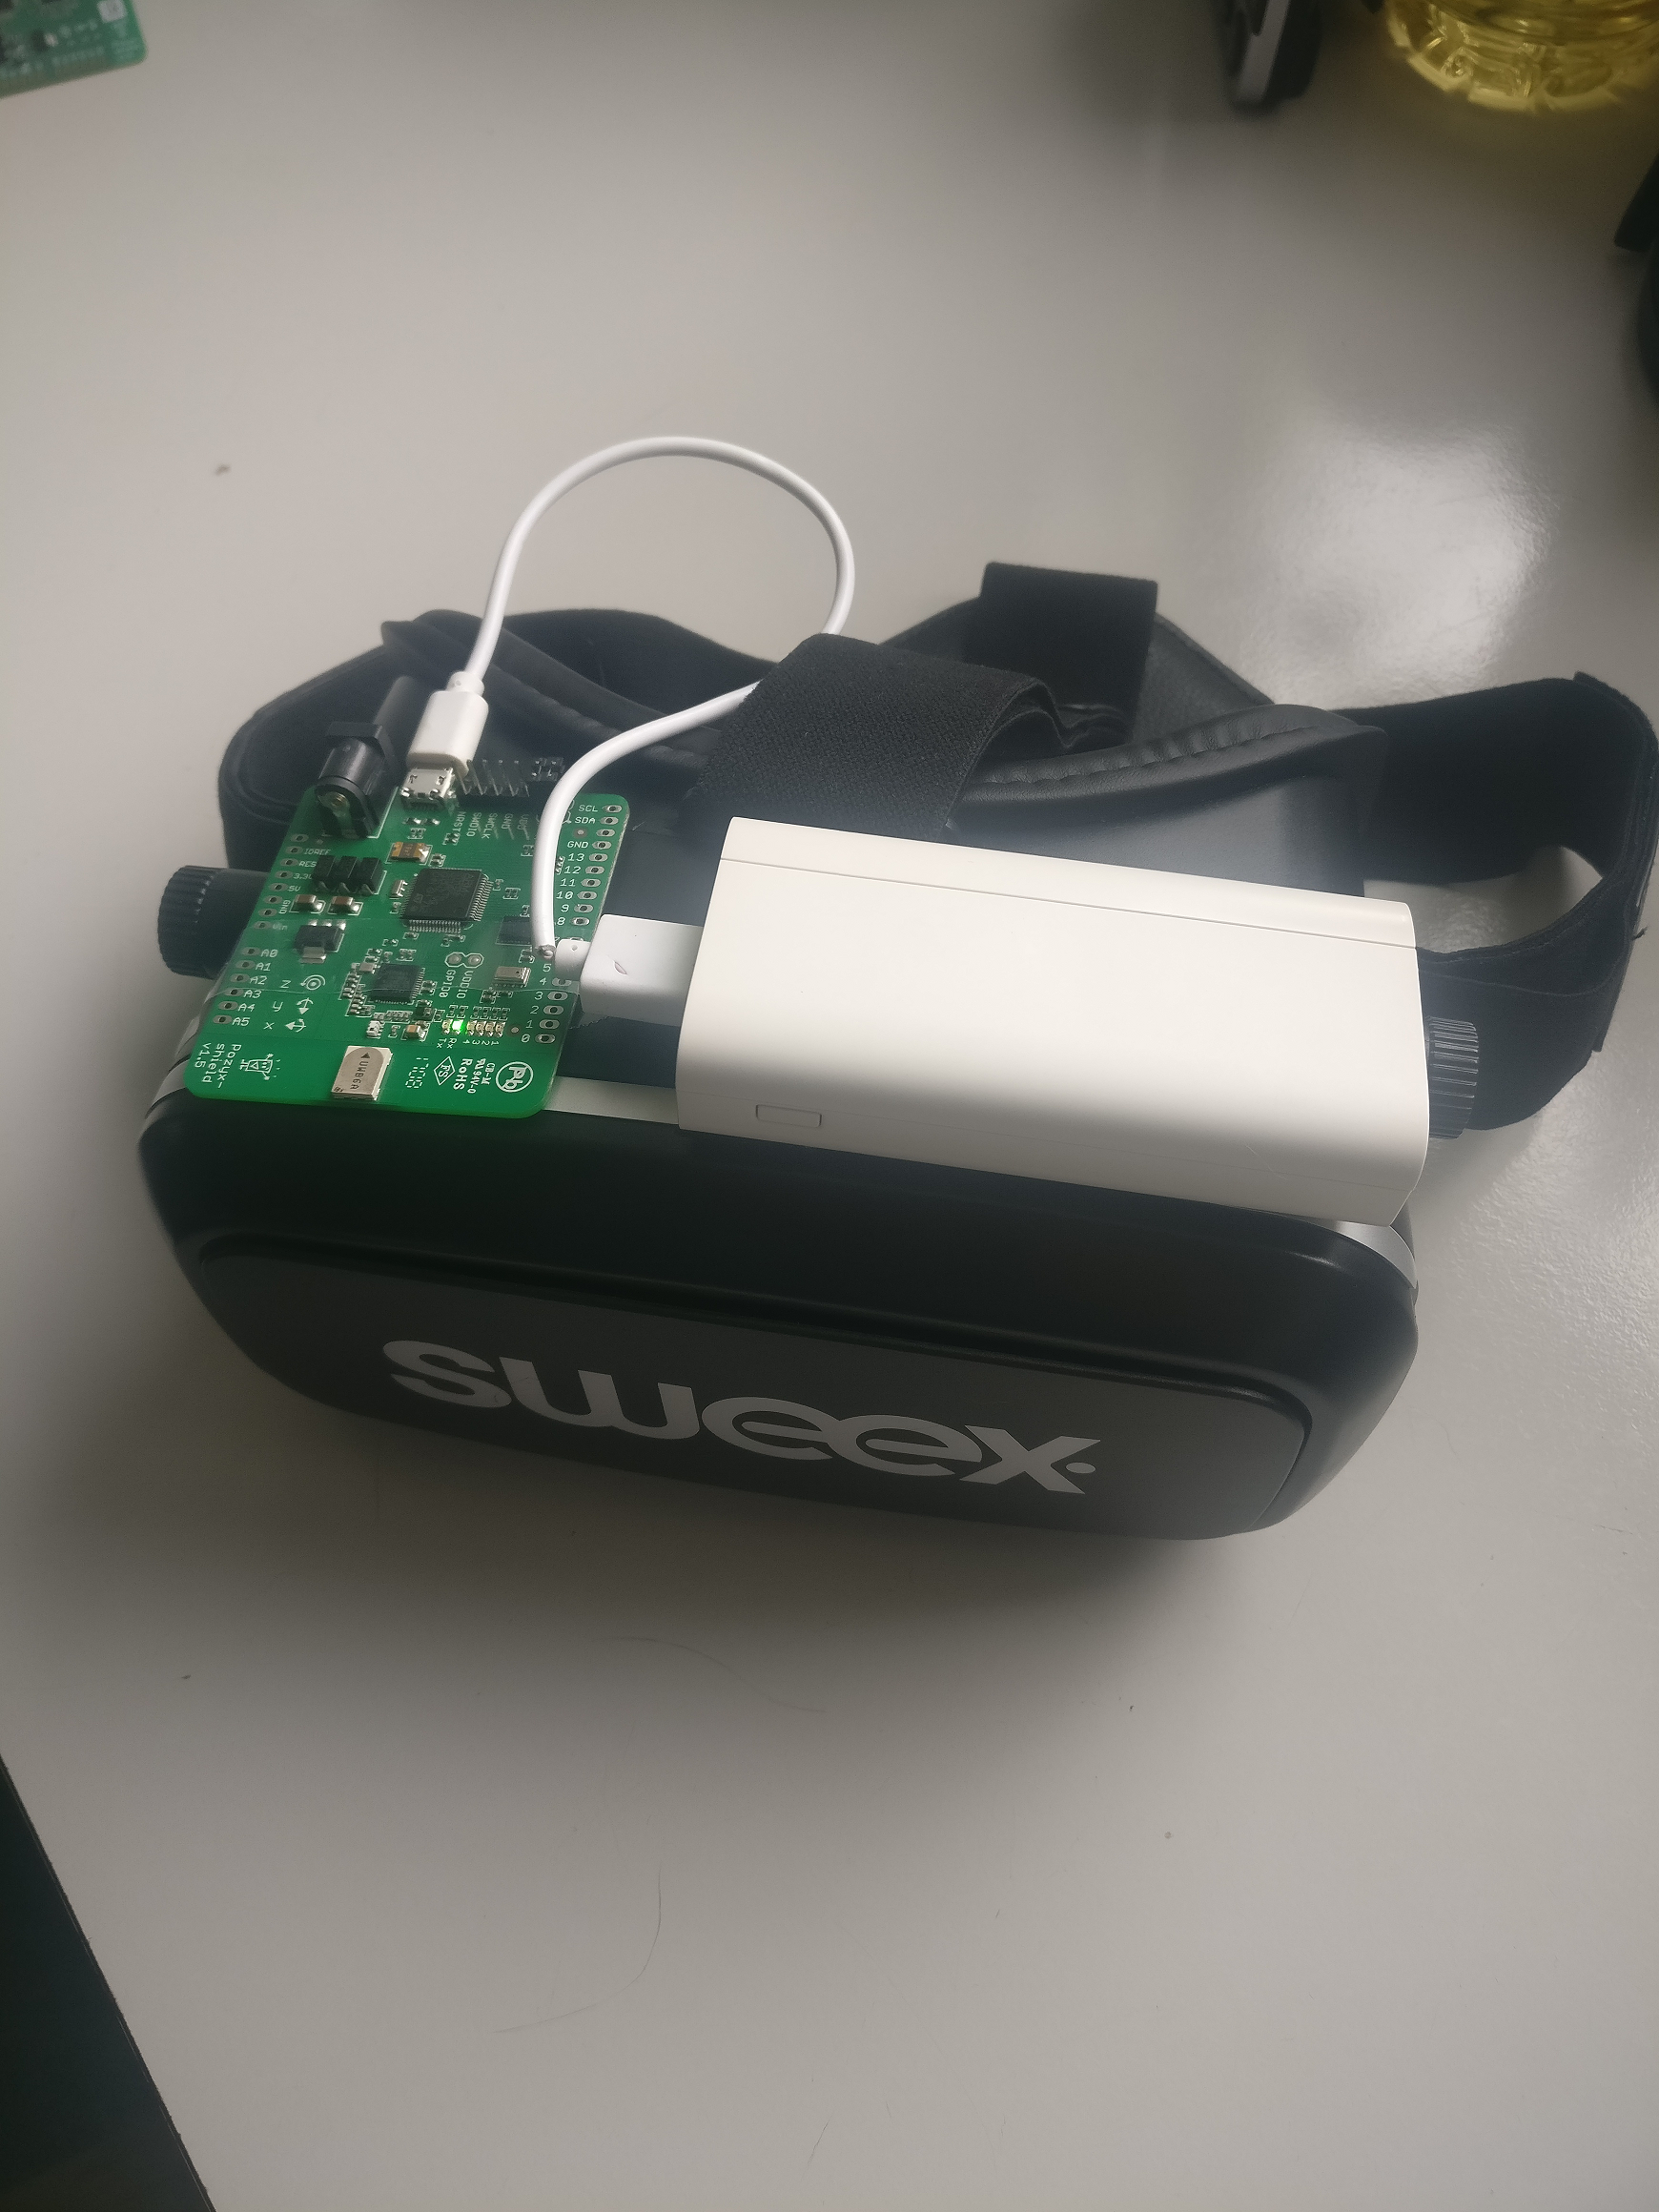
\includegraphics[width=0.4\linewidth]{usability/tagonvrheadset.png}
    \caption{Possible placement of Pozyx in future versions.}
    \label{fig:tag-on-vr-headset}
\end{figure}
\noindent
Finally, the problem with the update rate being slow is hard to fix, since it is a hardware limitation of Pozyx.
However, it would be possible to implement dead reckoning to improve this as described in \autoref{sec:dead-reckoning}.
